\section{Megvalósítás}
\subsection{Használt erőforrások}
A háló összerakást saját gépen kezdtük el. Majd a véglegesítését és a tanításokat AWS szerveren, NVIDIA Tesla K80 12GB videokártyán végeztük. Jupyter notebook-ban futtatuk a tanításokat, kerasban felépített hálóval\ [5], ezek elmentett adatait aztán Tensorboard segítségével elemeztük\ [7].
\subsection{Fejlesztés}
A fejlesztés során scriptet írtunk az adatok generálására( {\it generate\_dataset.py}). Ez állítja elő a tiszta adatfájlokból a hálók bemeneteit.

A különböző hálókat jupyter notebookokban teszteltük. Ezek a {\it model} kezdetű notebookokban találhatóak.

A végső eredményeket a {\it results} notebookban összegeztük, ez végigfuttatható demonstrációként hamar előáll. 
\subsection{Eredmények}
Zöngésség becslésére nagyon jó, alapfrekvencia (pitch érték) meghatározására használhatóan jó és a spektrális paraméter (Mel-Cepstrum) jósolására kezdetleges eredményeket sikerült elérnünk. (utóbbiról ezért nem is mellékeltünk tanítási és validációs grafikonokat). Hiperparaméter optimalizálás tekintetében egyelőre kézzel dolgoztunk (ez még javításra szorul), már így is sikerült használható pontosságot  elérnünk.

\textit{(A grafikonok y tengelyén az MSE hiba értéke x tengelyén az elvégzett epoch-ok száma látható.)}

\subsubsection{Zöngésség}
	Zöngésség becslése egyszerűbb, futásidő tekintetében gyorsabb feladatnak bizonyult. Ezért itt nem alkalmaztunk early stopping-ot, hanem a több próbálkozás után a fixen 410 epoch-kal történő tanításnál maradtunk.
	
	A teszt adatainkon elért eredmények:
	
	pontosság 0.8342
	
	költségfüggvény: 0.1560
	
	\textit{(MSE hiba értékekkel számítva)}

\begin{figure}[h]
	\par\centering
	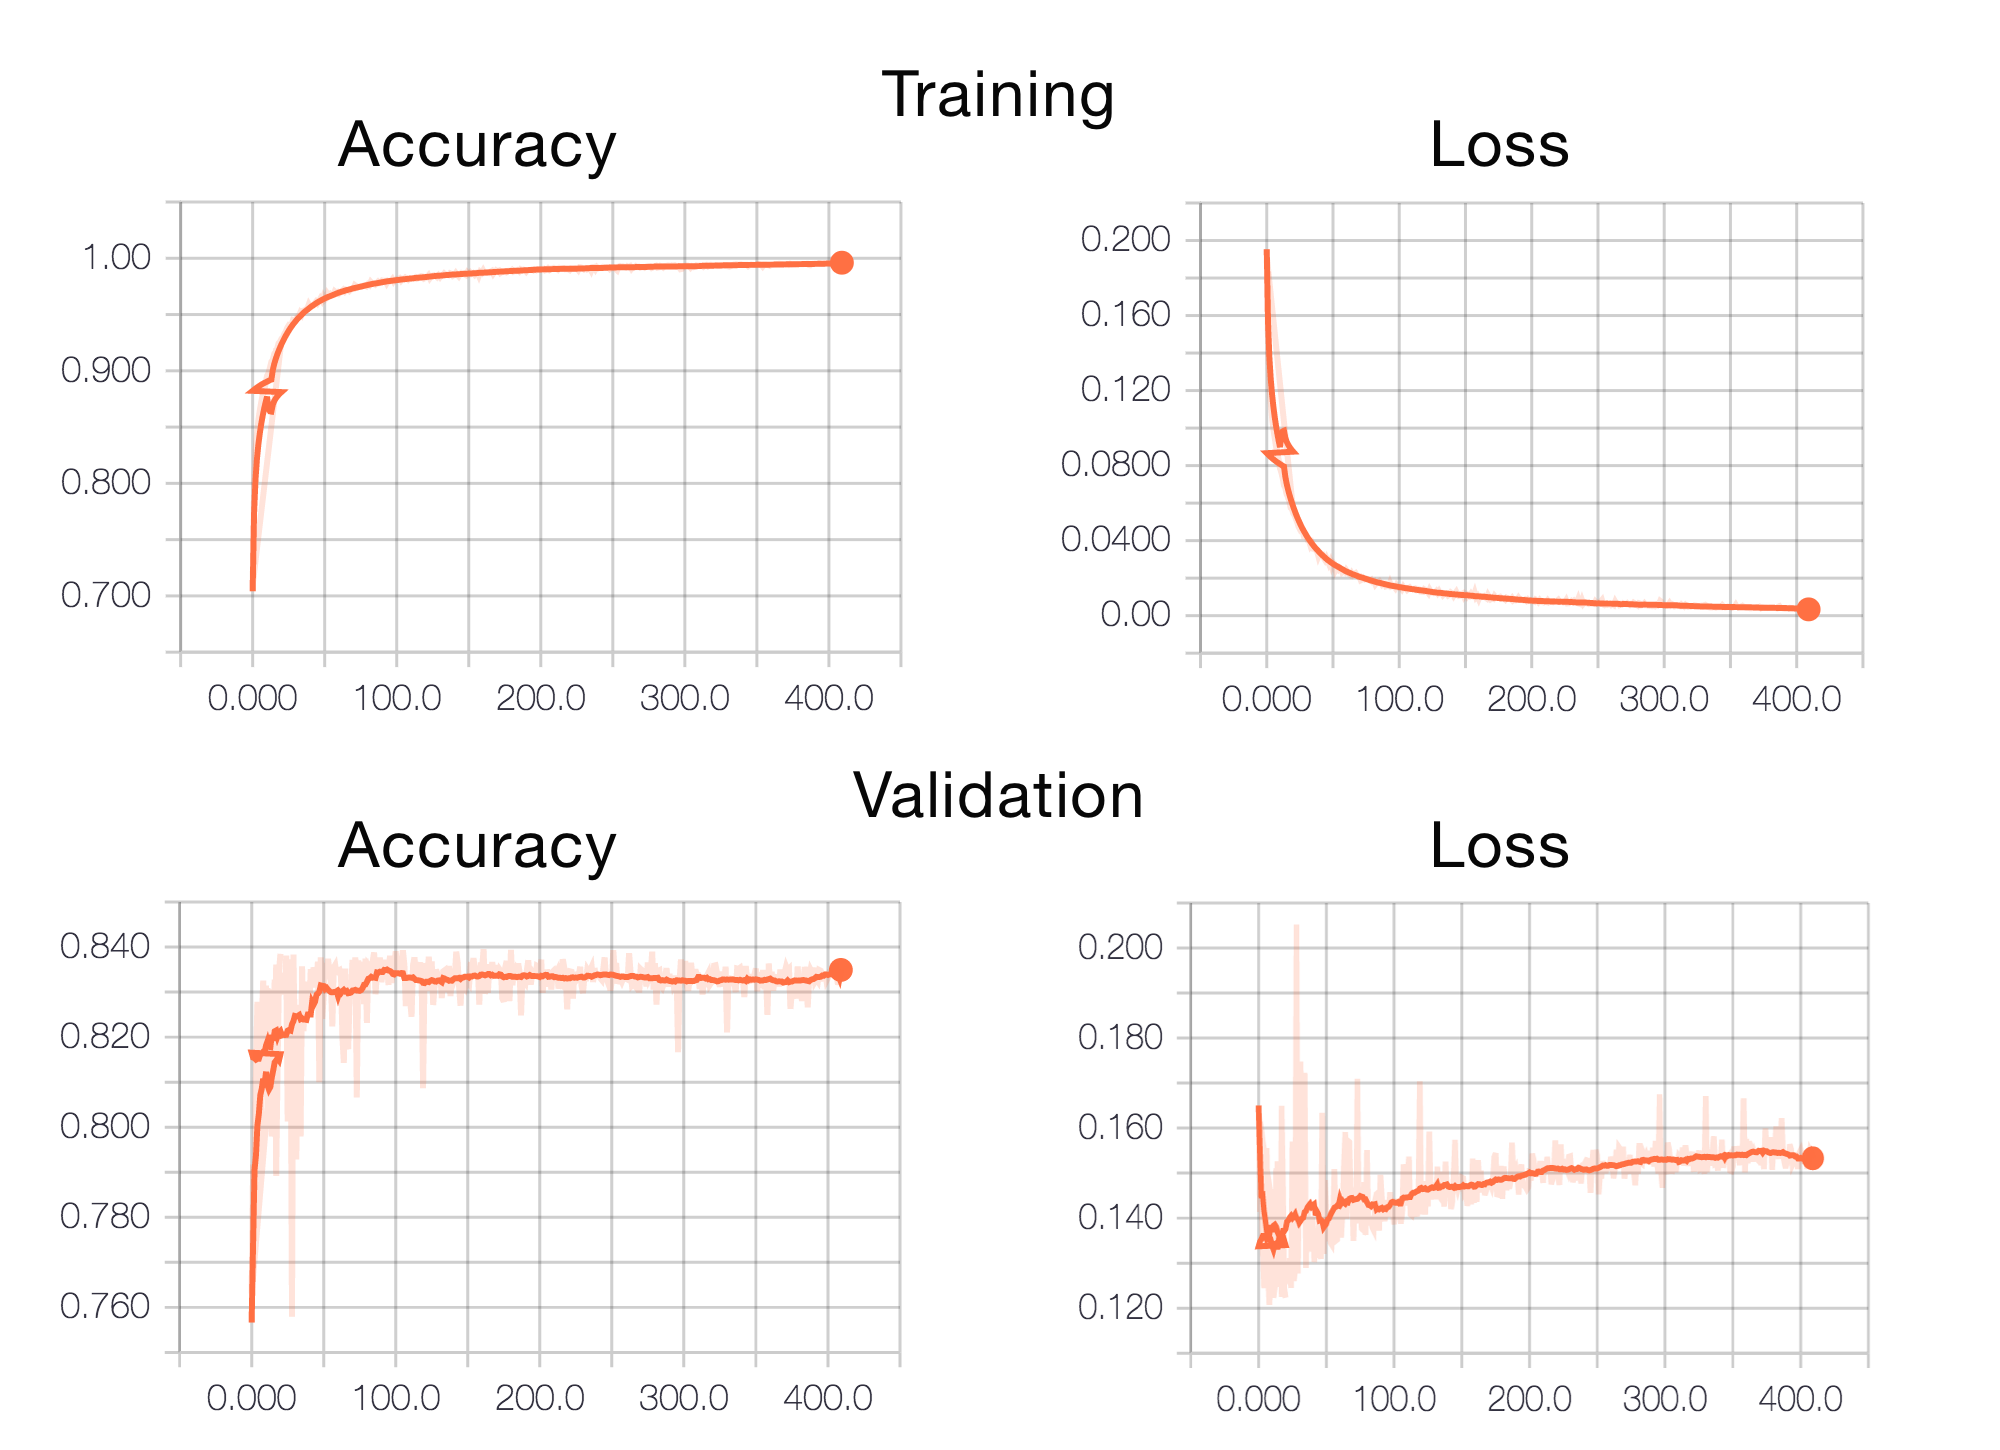
\includegraphics[width=0.65\textwidth,keepaspectratio]{uv_fig}
	\caption{Zöngésség tanítás}
\end{figure}

\subsubsection{Alapfrekvencia}
Az alapfrekvencia tanítása esetén alkalmaztunk early stoppig-ot. Ez azonban (a paramétereinek állítása után is) túl hamar állt meg. Ennek következtében több tanítást is elvégeztünk egymás után. Az itt kapott eredményeink messze nem olyan szépek mint a zöngésségé, de ezek is használhatónak bizonyultak.

A teszt adatainkon elért eredmények:

pontosság: 0.4243

költségfüggvény: 0.07214

\textit{(MSE hiba értékekkel számítva)}
\begin{figure}[h]
	\par\centering
	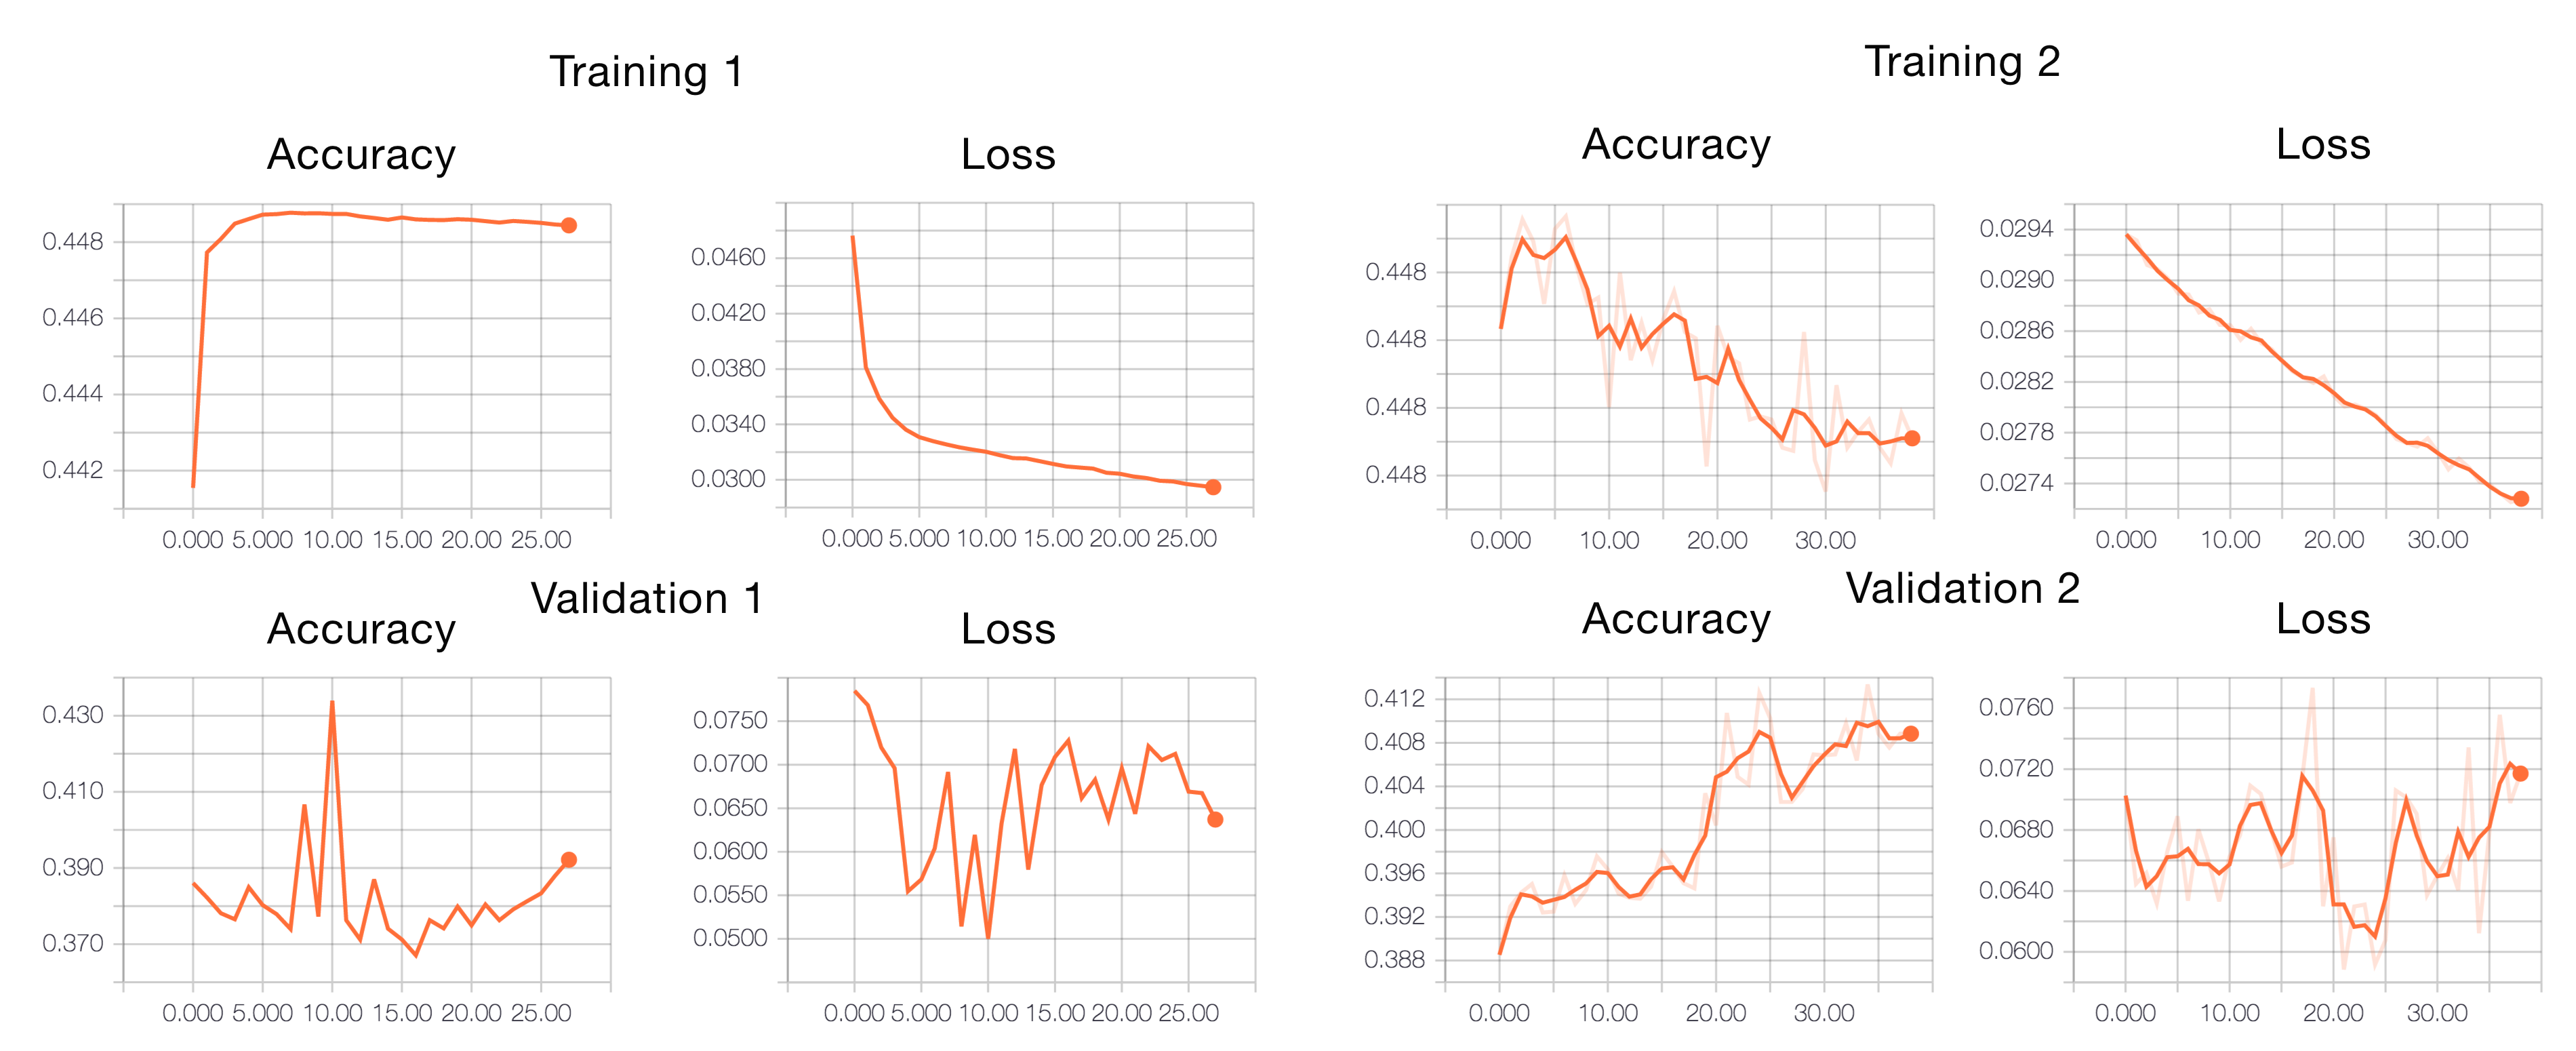
\includegraphics[width=\textwidth,keepaspectratio]{pitch_fig}
	\caption{Pitch tanítás}
\end{figure}
\subsubsection{MC paraméterek}
MC tanításakor kiütközött, hogy a bemeneti paramétereink nagyon megegyezőek voltak fonémán belül, így darabos lett a tanítás. Ez a magasabb MC értékekre jelentős hibát okozott, így megpróbáltuk kevesebb mc érték használatát pontosítani.

	
	A teszt adatainkon elért eredmények:
	
	pontosság 0.2927
	
	költségfüggvény: 0.2086
	
	\textit{(MSE hiba értékekkel számítva)}
\begin{comment}
Innen hiányzik egy kép
\begin{figure}[h]
	\par\centering
	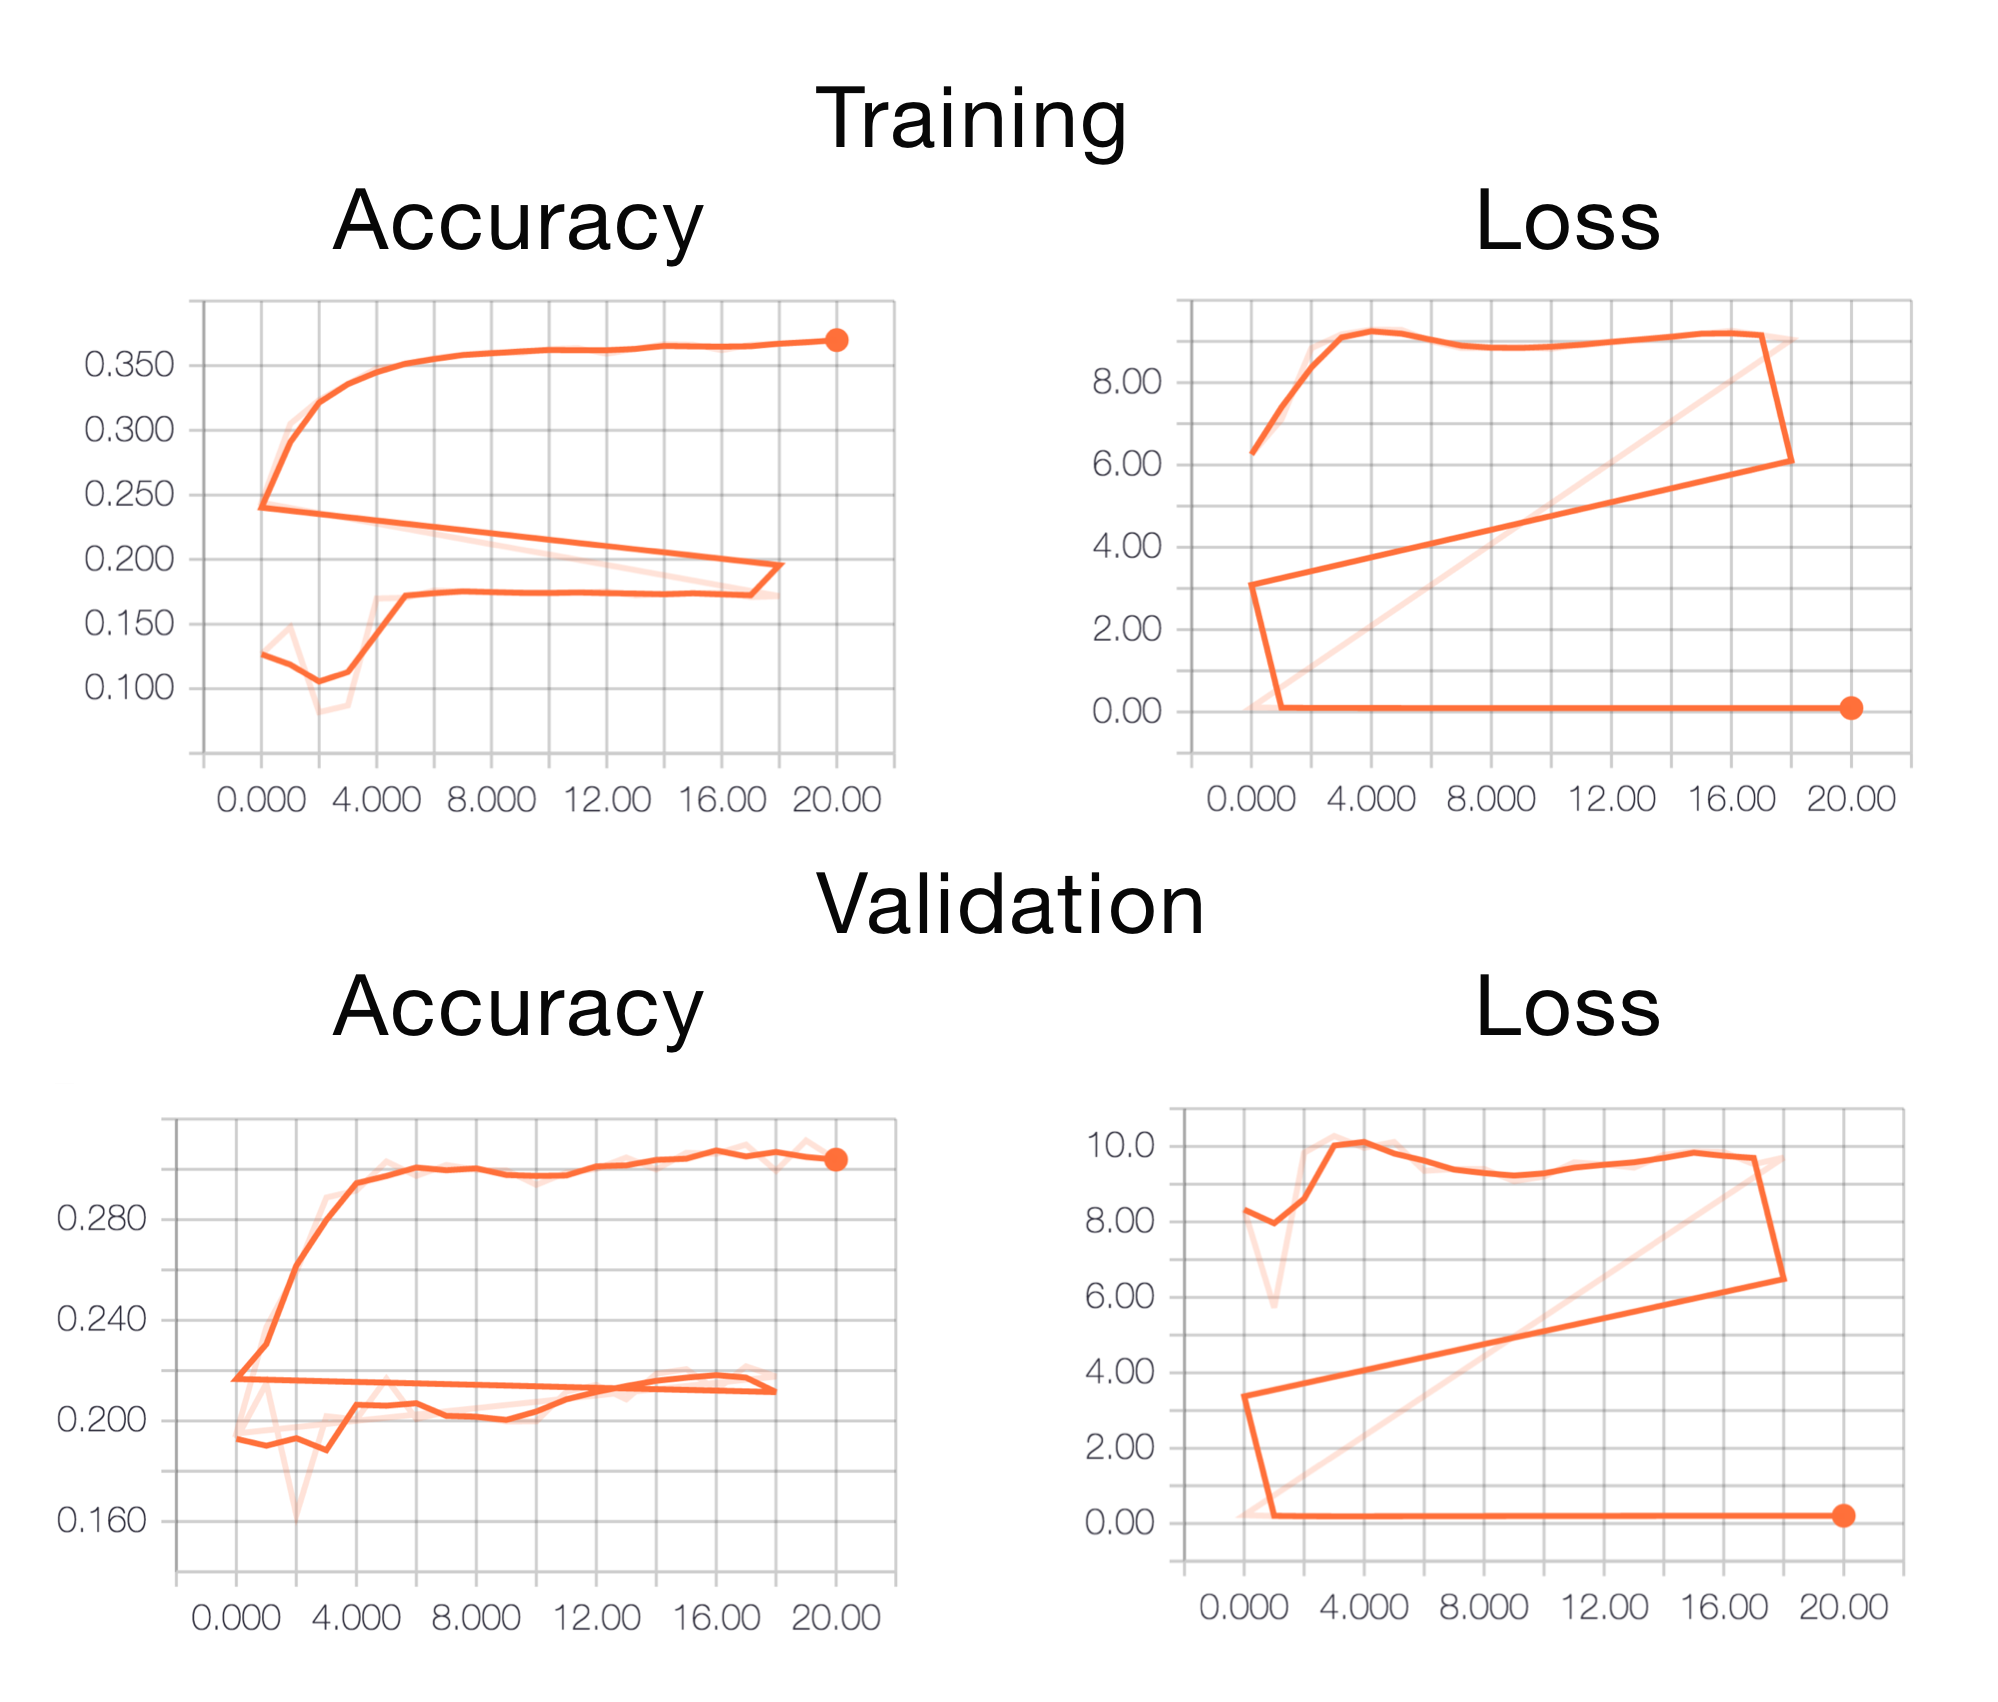
\includegraphics[width=0.8\textwidth,keepaspectratio]{length_fig}
	\caption{MC paraméterek tanítása}
\end{figure}
\end{comment}
\subsubsection{Fonéma hossz}
Fonéma hossz becslésnél csoportosítást valósítottunk meg, a fonémákat 8 csoportba osztottuk, a csoportok között 12,5 ms eltéréssel és a csoportra végeztünk classificationt. Erre azért volt szükség mivel viszonylag kevés, géppel annotált tanító adat állt a rendelkezésünkre, ezek alapján nem sikerült használható eredményeket elérni(1000 mondat, kb. 16000 fonéma ami átlagosan egy fonémára 400 mintát jelent, de ez nem egyenletes így előfordulhat olyan fonéma amire ennél jóval kevesebb tanítóadat szerepel). 

Az adatokban szereplő eredeti hosszak vizsgálata után ezt a csoportosítási módot választottuk, két szempont a megfelelő differenciálódás és a jelentősen kilógó adatok levágása volt. Tehát minden fonémánk 40 és 140 ms közé került. (A tanító adatainkat is ez alapján módosítottuk még a feldolgozási fázisban, minden keretnél hosszabb fonémát 140 ms-nél levágunk.)


A teszt adatainkon elért eredmények:
	
pontosság 0.4619
	
költségfüggvény: 0.02419
	
\textit{(MSE hiba értékekkel számítva)}

\begin{figure}[h]
	\par\centering	
	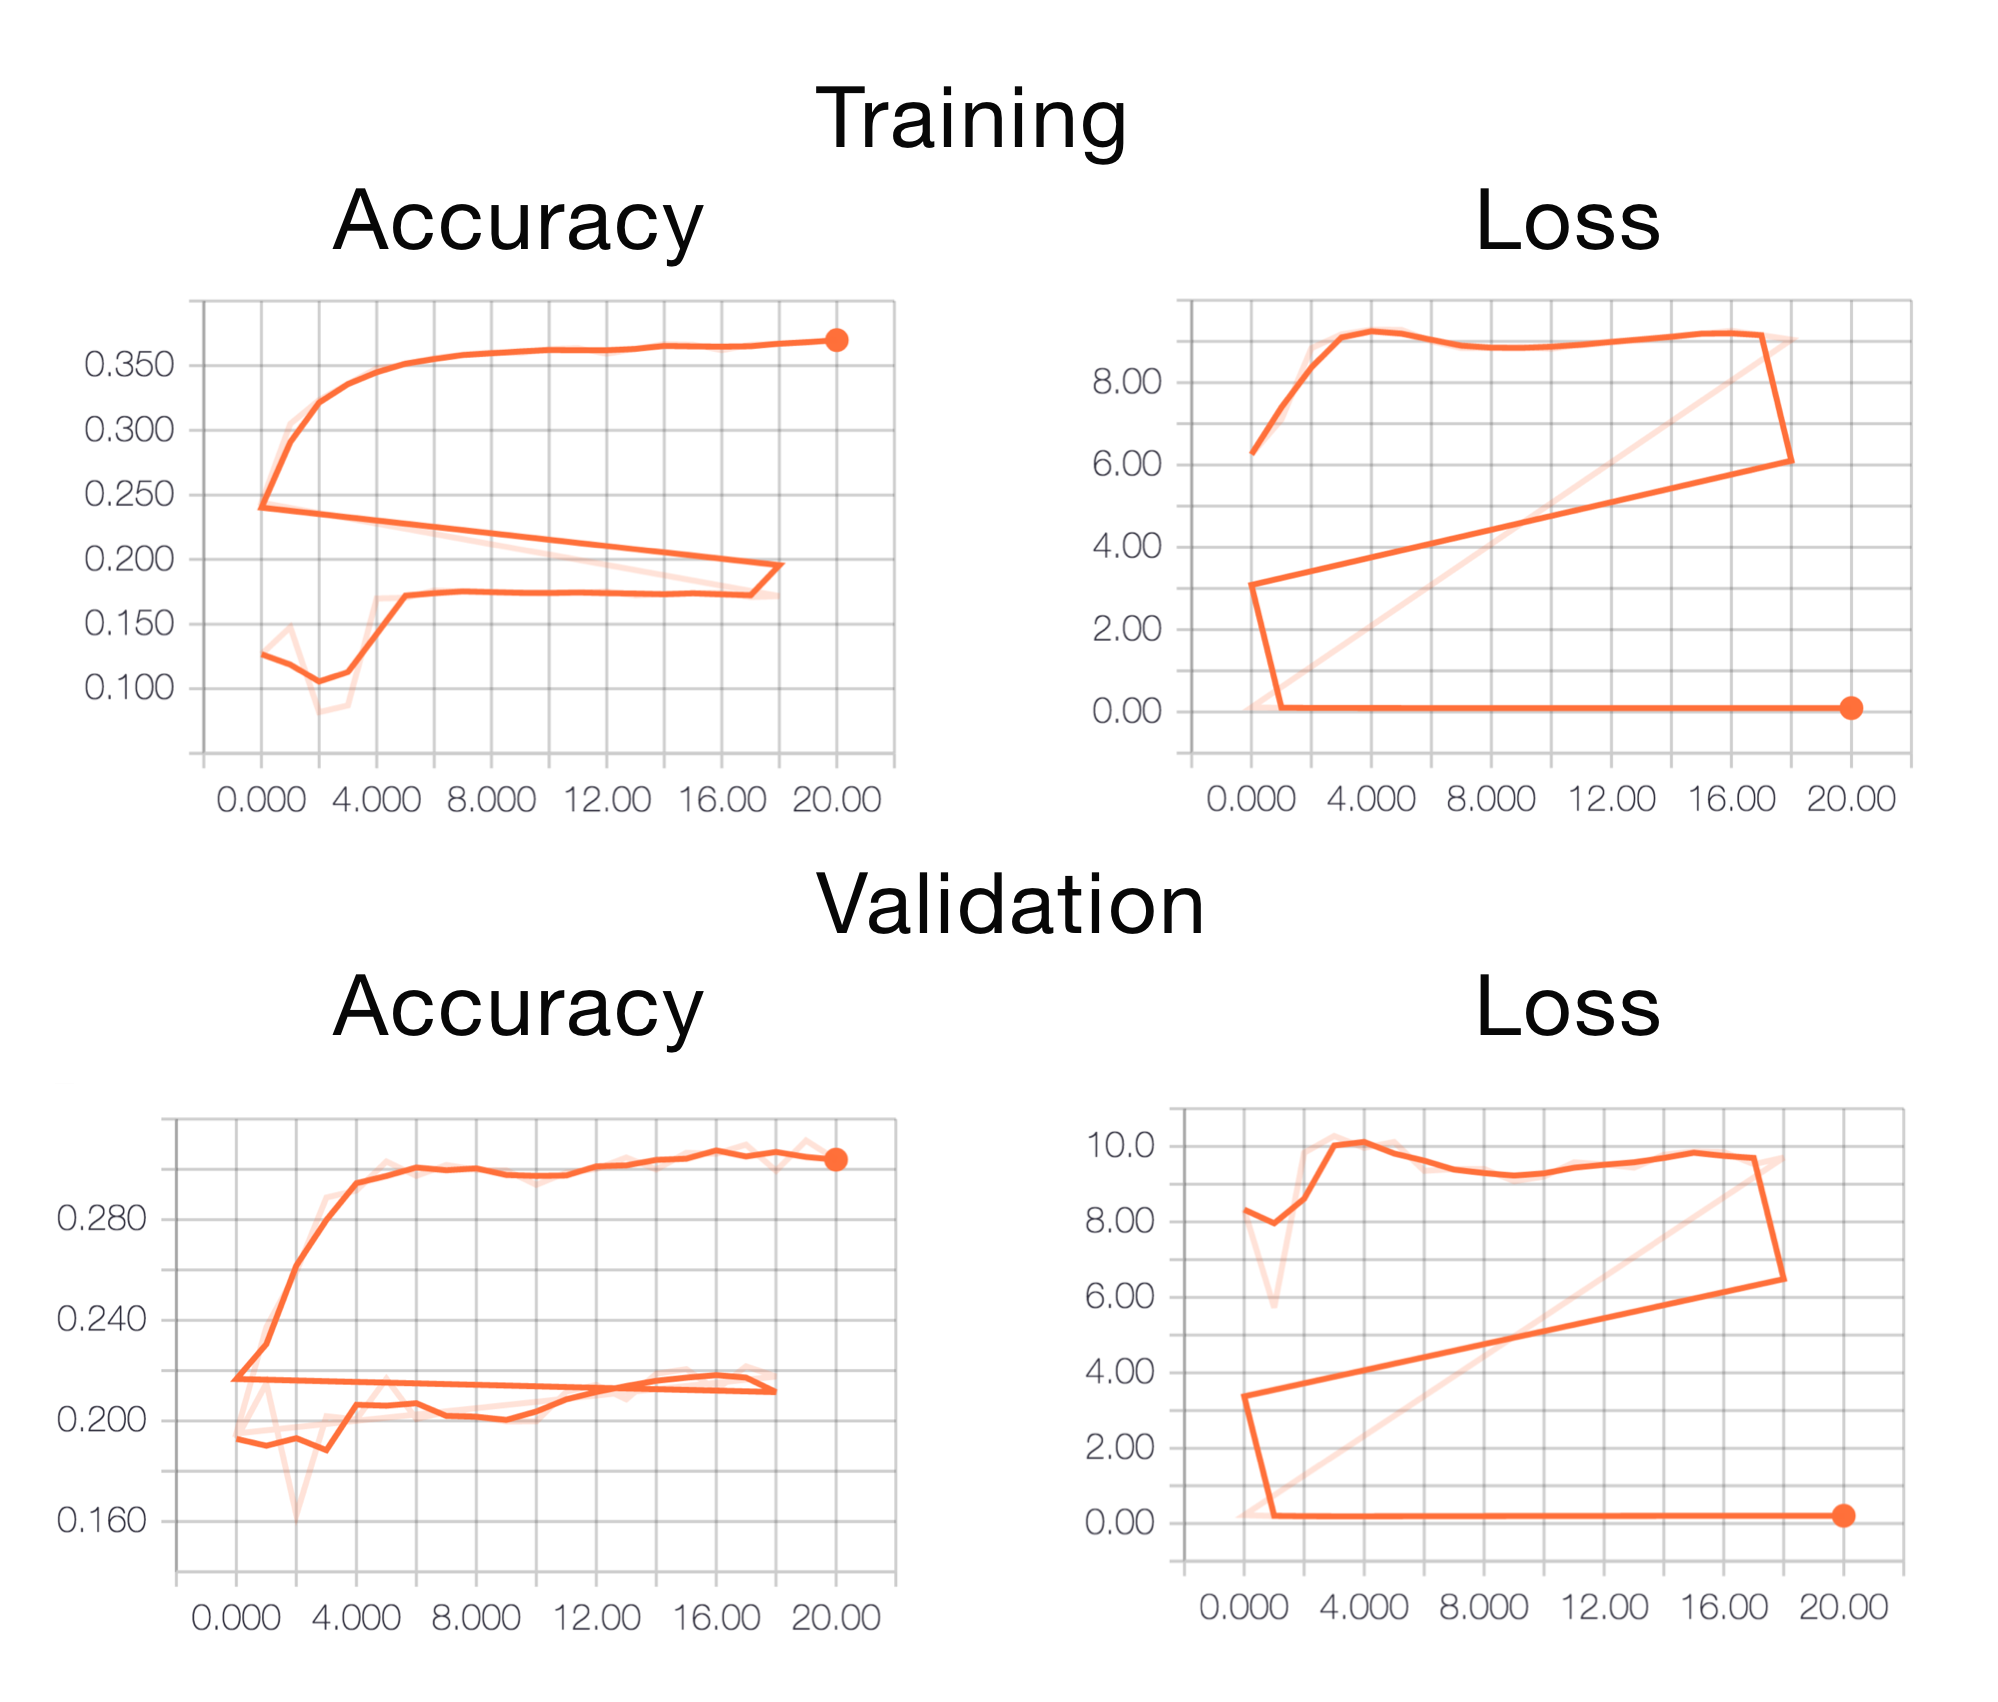
\includegraphics[width=0.7\textwidth,keepaspectratio]{length_fig}
	\caption{Fonéma hossz tanítás}
\end{figure}
\subsubsection{Teljes becslő}
A fenti paraméterek ismeretében teljes TTS végezhető. 

A mondat alapján fonéma hosszakat becslünk, majd párhuzamosan zöngésség-alapfrekvencia és mc paraméter becslés folyik, végül a kapott eredményekből előállítható a kimenet.
\clearpage
\subsection{Eredmények egy példán bemutatva}
Az alábbi {\it"But all my dreams violated this law"} mondaton elvégezve a becslést:
\subsubsection{Adatok beolvasása}
Az adatok beolvasása egy eredeti hangfájlból (\ref{law-1}.ábra), majd a csöndek szűrése és a pitch-MC paraméterek előállítása(\ref{law-2}.ábra).
\begin{figure}[h]
	
	\par\centering	
	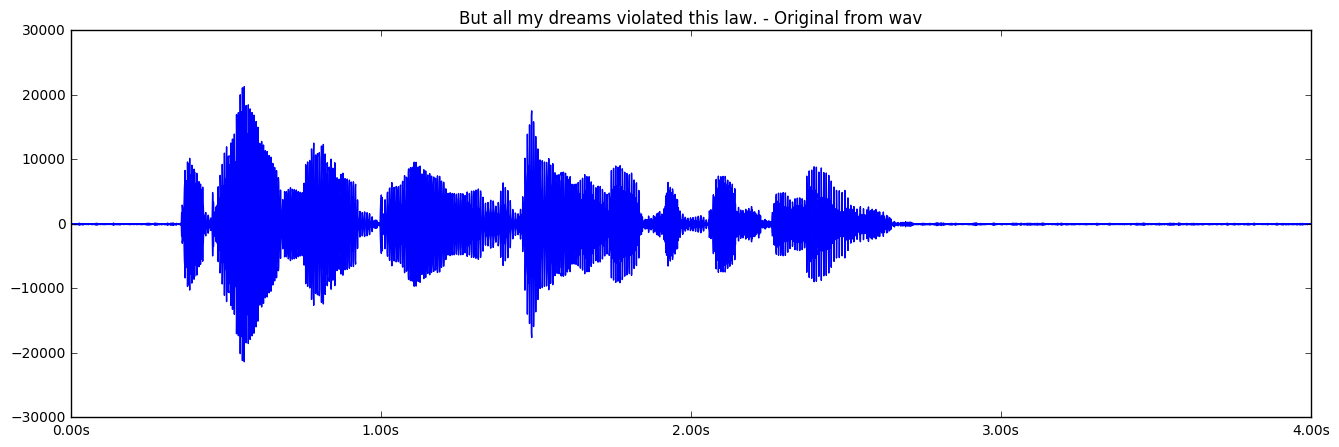
\includegraphics[width=\textwidth,keepaspectratio]{law_in}
	\caption{Beolvasott hangfájl}
	\label{law-1}
\end{figure}
\begin{figure}[h]
	\par\centering	
	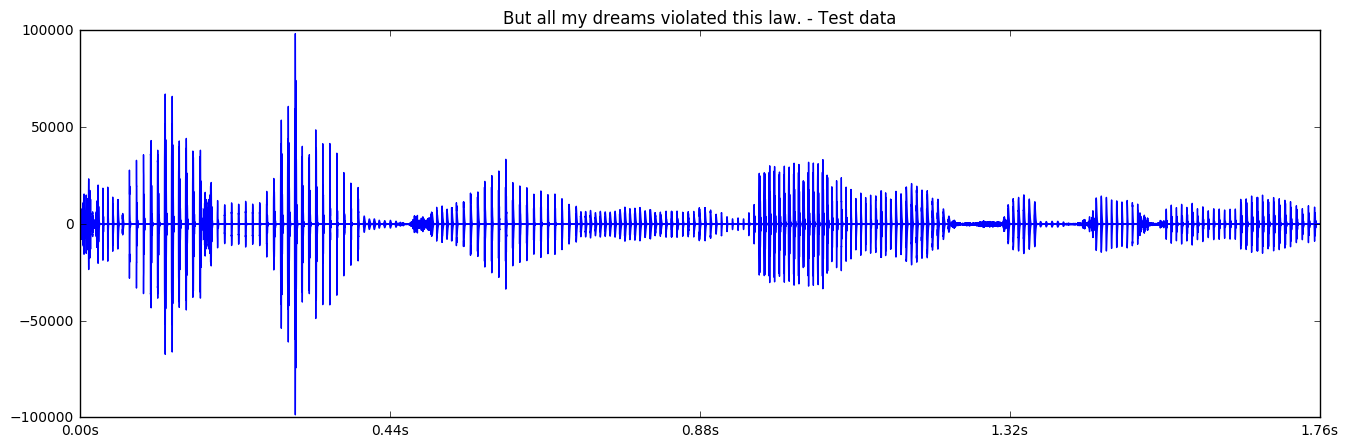
\includegraphics[width=\textwidth,keepaspectratio]{law_data}
	\caption{A hangfájl szűrve, MC-pitch értékek generálva PySPTK segítségével}
	\label{law-2}
\end{figure}
\subsubsection{Zöngésség becslés}
A zöngésség becslése jól működik.
\begin{figure}[h]
	
	\par\centering	
	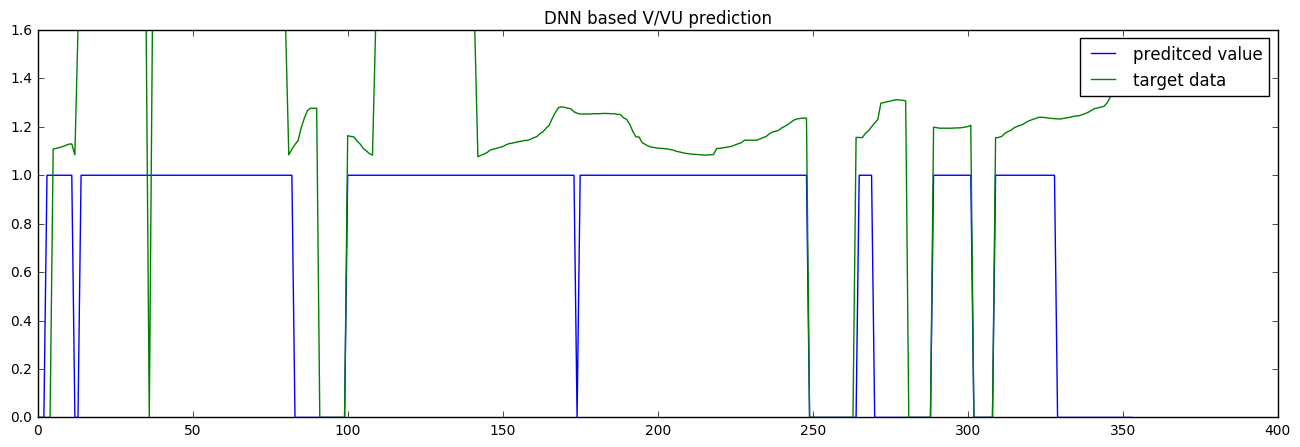
\includegraphics[width=\textwidth,keepaspectratio]{law_vuv}
	\caption{Beolvasott hangfájl}
\end{figure}
\subsubsection{Pitch becslés}
Alapfrekvencia becslése(\ref{law-3}. ábra), majd kimenet előállítása a tanult gerjesztési és a hozott spektrális paraméterekkel(\ref{law-4}. ábra). A \ref{law-5}. ábrán ugyanez látható a tanult zöngésség bevezetésével.
\begin{figure}[h]
	\par\centering	
	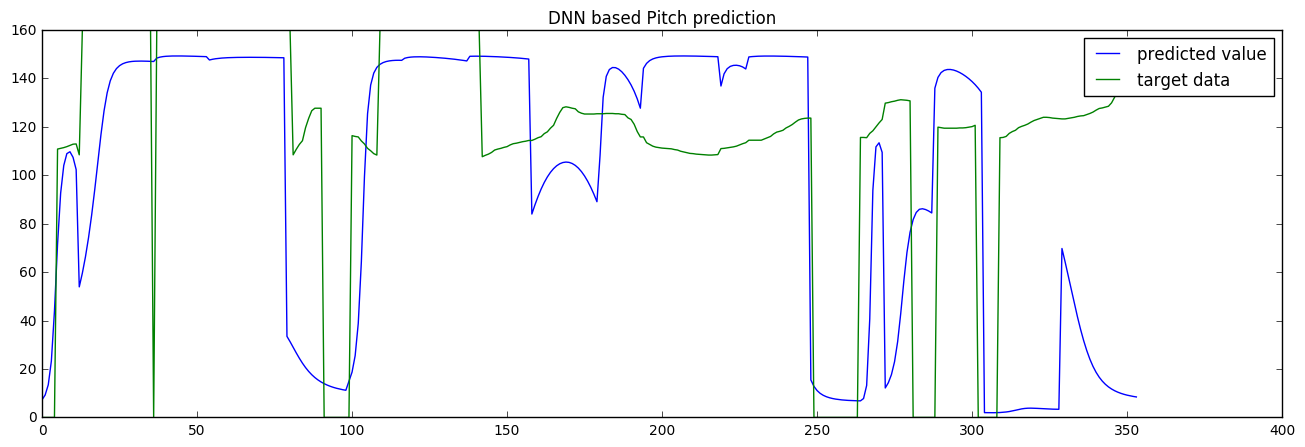
\includegraphics[width=\textwidth,keepaspectratio]{law_pitch}
	\caption{F0 becslése}
		\label{law-3}
\end{figure}
\begin{figure}[h]
	\par\centering	
	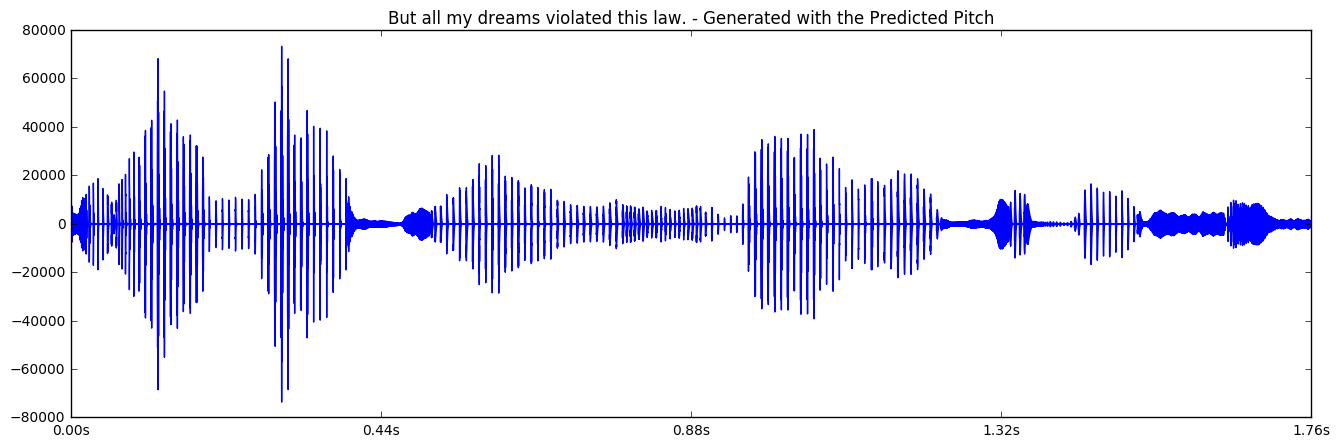
\includegraphics[width=\textwidth,keepaspectratio]{law_pitch_wav}
	\caption{Generált hang F0 becsléssel, MC az eredeti hang alapján}
		\label{law-4}
\end{figure}
\begin{figure}[h]
	\par\centering	
	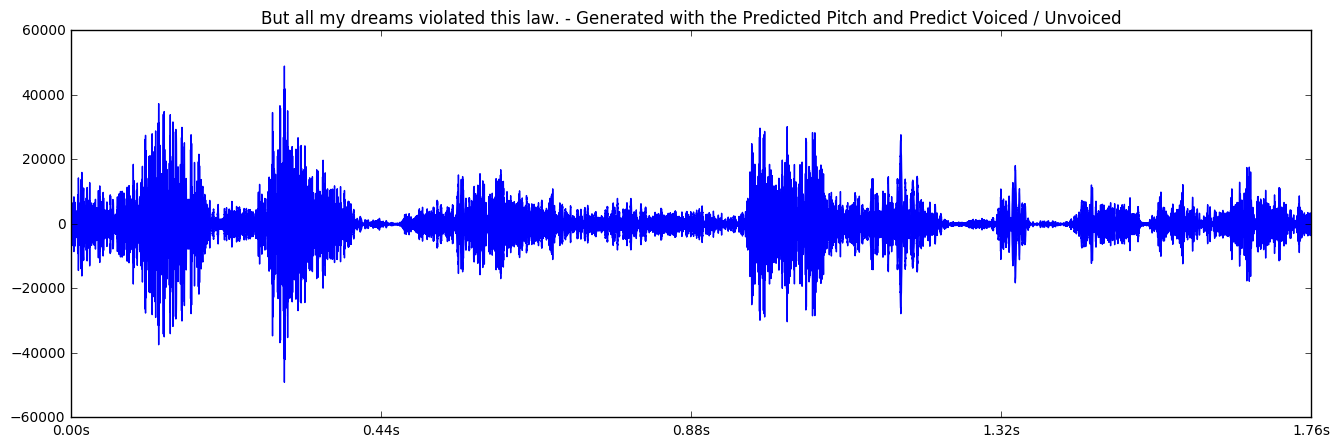
\includegraphics[width=\textwidth,keepaspectratio]{law_pitch_vuv}
	\caption{Generált hang F0 és V/UV értékek alapján}
		\label{law-5}
\end{figure}

\clearpage
\subsubsection{MC becslés}
Az MC becslőnél a görbe sajnos meglehetősen lépcsősen illeszkedik (\ref{law-6}. ábra), és ez a generált hangon is érezhető (\ref{law-7}. ábra).
\begin{figure}[h]
	\par\centering	
	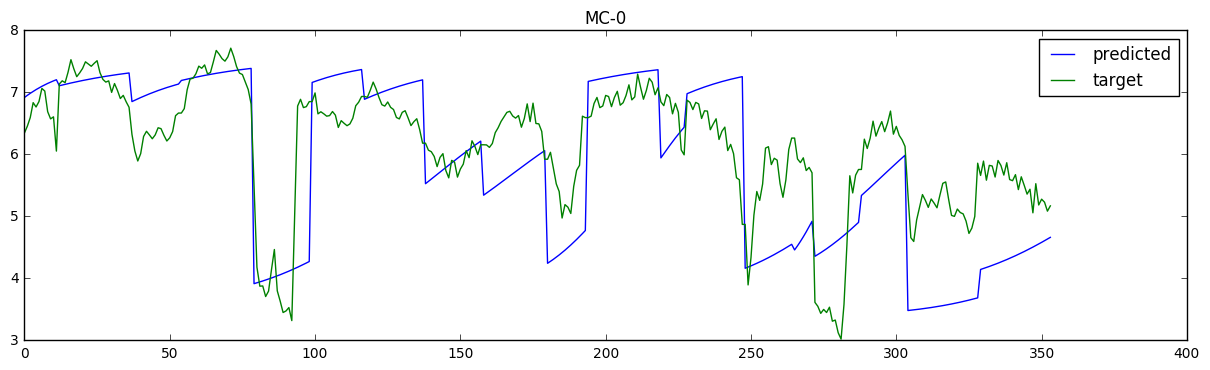
\includegraphics[width=\textwidth,keepaspectratio]{law_mc_0}
	\caption{MC-0 becslése}
	\label{law-6}
\end{figure}
\begin{figure}[h]
	\par\centering	
	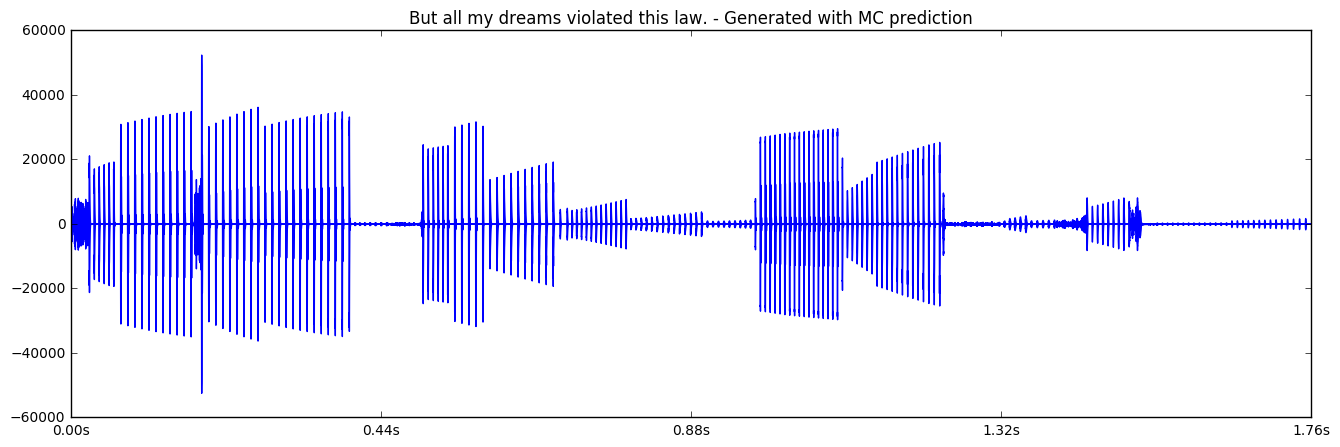
\includegraphics[width=\textwidth,keepaspectratio]{law_mc}
	\caption{Generált hang hozott F0-val és becsült MC értékekkel}
	\label{law-7}
\end{figure}
\subsubsection{Hanggenerálás tanult F0 és MC értékekkel}
A végleges generált hangból sajnos nem lehet kivenni az eredeti szavakat(\ref{law-8}. ábra).
\begin{figure}[h]
	\par\centering	
	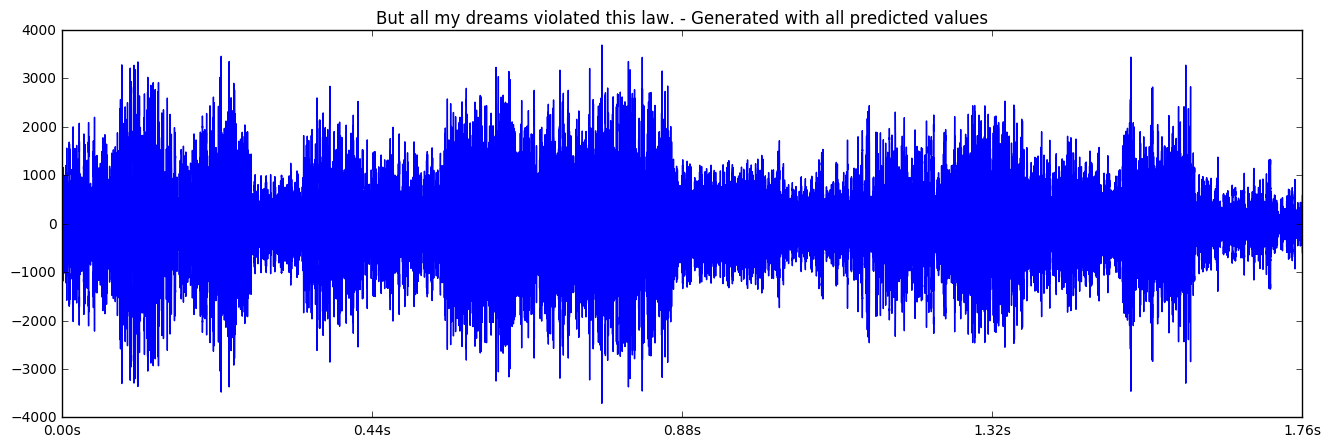
\includegraphics[width=\textwidth,keepaspectratio]{law_end}
	\caption{Generált hang becsült F0-val és MC értékekkel}
	\label{law-8}
\end{figure}